%!TEX root = ./main.tex

\setcounter{section}{4}
\setcounter{equation}{56}
\newcommand{\likpri}[1]{p(\vx\given\cC_{#1})p(\cC_{#1})}

\section*{4.2 確率的生成モデル}


\begin{align}
p(\cC_1\given\vx) & = \frac{\likpri{1}}{\likpri{1} + \likpri{2}} \notag \\
& = \frac{1}{1 + \exp(-a)} \notag \\
& = \sigma(a)
\end{align}
ここで $a$ を
\begin{equation}
  a = \ln \frac{\likpri{1}}{\likpri{2}}
\end{equation}
と定義した.

\paragraph{シグモイド関数}
$\sigma(\cdot)$ は\emph{シグモイド関数 (logistic sigmoid function)}と呼ばれる関数.
\begin{equation}
\sigma(z) = \frac{1}{1 + \exp(-z)}
\end{equation}

\begin{itemize}
  \item 入力 $z$ を区間 $[0, 1]$ に押し込んで出力するので,なんらかの計算を行った最後で確率を出力したい時によく出てくる.(e.g. ロジスティック回帰,ニューラルネットワーク)
  \item 対称性がある
  \begin{equation}
    \sigma(-z) = 1 - \sigma(z)
  \end{equation}
  \item 逆関数は \emph{ロジット関数 (logit function)} として知られている(統計学の世界ではリンク関数,i.e. 活性化関数の逆関数, を考えることが多い).
  \begin{equation}
    z = \mathrm{logit}(\sigma) = \ln \parens{\frac{\sigma}{1-\sigma}}
  \end{equation}
\end{itemize}

\newpage
ロジスティック関数を他クラスに拡張したものは \emph{ソフトマックス関数 (softmax function)} として知られている.
\begin{align*}
  \vz \in \R^M,\, \vs(\vz) & = \left(\begin{array}{c}
    s_1(\vz) \\
    \vdots \\
    s_{M}(\vz)
    \end{array}\right) \\
  s_i(\vz) & = \frac{\exp(\vz_i)}{\sum_j \exp(\vz_j)}
\end{align*}

\begin{equation}
  p(\cC_k \given \vx) = \frac{\likpri{k}}{\sum_j \likpri{j}} = s_k(\ln \likpri{k})
\end{equation}


\subsection*{4.2.1 連続値入力}

クラスの条件付き確率 $p(\vx \given \cC_k)$ がガウス分布であると仮定して,事後確率がどうなるかを考える.
すべてのクラスが同じ共分散行列を共有していると仮定する.
\[
p(\vx \given \cC_k) = \parens{2\pi}^{-\frac{D}{2}} \abs{\mSigma}^{-\frac{1}{2}} \exp \braces{-\frac{1}{2} (\vx - \vmu_k)^\top \mSigma^{-1} (\vx - \vmu_k) } \tag{4.64}
\]

\subsubsection*{2クラス}

\begin{equation}
  p(\cC_1 \given \vx) = \sigma(\vx^\top \vx + w_0)
\end{equation}
\begin{align}
  \vw & = \mSigma^{-1} (\vmu_1 - \vmu_2) \\
  w_0 & = -\frac{1}{2} \vmu_1^\top \mSigma^{-1} \vmu_1 + \frac{1}{2} \vmu_2^\top \mSigma^{-1} \vmu_2 + \ln \frac{p(\cC_1)}{p(\cC_2)}
\end{align}

\begin{itemize}
  \item シグモイド関数の中身が $\vx$ の線形関数である(i.e. 境界面 $\sigma(\cdot) = 0.5 \iff \vx^\top \vx + w_0 = 0$ が 入力空間において線形).
  \item 事前分布バイアスパラメータ $w_0$ にしか影響しない(i.e. 境界面を平行移動させるだけ).
\end{itemize}

\subsubsection*{Kクラス}

\begin{align}
  p(\cC_k \given \vx) & = \mathrm{softmax}_k(a_k) \notag \\
  & =  \mathrm{softmax}_k( \vw_k^\top \vx + w_{k0} )
\end{align}
\begin{align}
  \vw_k & = \mSigma^{-1} \vmu_k \\
  w_{k0} & = -\frac{1}{2} \vmu_k^\top \mSigma^{-1} \vmu_k + \ln p(\cC_k)
\end{align}

\begin{itemize}
  \item $a_k$ が $\vx$ の線形関数となる.
  \item 誤分類率をロス関数とした場合(正解クラスに依らず,分類に成功したとき/失敗した時に課せられるペナルティが全て同じ場合)の境界面は,やはり $\vx$ の線形関数.
\end{itemize}

\setcounter{equation}{70}
\subsection*{4.2 最尤解}

クラスの条件付き確率 $p(\vx \given \cC_k)$ にパラメトリックな関数を定めると,クラスの事前確率 $p(\cC_k)$ とともに,パラメータの値を最尤法を用いて決めることができる.

\subsubsection*{2クラス}

$\vx_n \in \R^M,\, t_n \in \set{0,1}$ な訓練集合 $\cD \defeq \set{\vx_n, t_n}_{n=1}^N$ が与えられている.
\begin{itemize}
  \item $t_n = 0 \implies \vx_n$ はクラス $\cC_1$
  \item $t_n = 1 \implies \vx_n$ はクラス $\cC_2$
\end{itemize}

ここで,クラスの事前分布を $p(\cC_1) = \pi,\, p(\cC_2) = 1 - \pi$ とすると,尤度関数は
\begin{align}
  p(\cD \given \pi, \vmu_1, \vmu_2, \mSigma) & = \prod_n \braces{\pi p(\vx \given \cC_1)}^{t_n} \braces{(1 - \pi) p(\vx \given \cC_2)}^{1 - t_n} \notag \\
  & = \prod_n \braces{\pi \cN(\vx_n \given \vmu_1, \mSigma)}^{t_n} \braces{(1 - \pi) \cN(\vx_n \given \vmu_2, \mSigma)}^{1 - t_n}
\end{align}

\paragraph{$\pi$ の最尤推定}

対数尤度 $\ln L(\pi, \vmu_1, \vmu_2, \mSigma)$ で $\pi$ が関係しているのは
\begin{equation}
   = \sum_n \braces{t_n \ln \pi + (1-t_n)\ln(1 - \pi)}
\end{equation}
なので,$\pp{\ln L}{\pi} = 0$ を解くと
\begin{equation}
  \pi = \frac{N_1}{N_1 + N_2}
\end{equation}
が得られる.ただし,$N_1,N_2$ はそれぞれ $\cC_1, \cC_2$ に属するデータの数.

\paragraph{$\vmu_1$ の最尤推定}

$\vmu_1$ が関係しているのは
\begin{equation}
  \sum_n t_n \ln \cN(\vx_n \given \vmu_1, \mSigma) = - \frac{1}{2} \sum_n t_n (\vx_n - \vmu_1)^\top \mSigma^{-1} (\vx_n - \vmu_1) + \mathrm{const.}
\end{equation}
なので,$\pp{\ln L}{\vmu_1} = 0$ を解くと
\begin{equation}
  \vmu_1 = \frac{1}{N_1} \sum_n t_n \vx_n
\end{equation}

$\vmu_2$ についても同様に解ける.
\begin{equation}
  \vmu_2 = \frac{1}{N_2} \sum_n (1 - t_n) \vx_n
\end{equation}

\paragraph{共分散行列の最尤推定}
$\mSigma$ が関係する項は以下の通り.
\begin{align}
  & - \fhalf \sum_n t_n \ln \abs{\mSigma} - \fhalf \sum_n t_n (\vx_n - \vmu_1)^\top \mSigma^{-1} (\vx_n - \vmu_1) \notag \\
  & - \fhalf \sum_n (1-t_n) \ln \abs{\mSigma} - \fhalf \sum_n (1-t_n) (\vx_n - \vmu_2)^\top \mSigma^{-1} (\vx_n - \vmu_2)  \notag \\ 
  & = -\frac{N}{2} \ln \abs{\mSigma} - \frac{N}{2} \Tr \braces{\mSigma\inv \vS} 
\end{align}
ここで,
\begin{align}
  \vS & = \frac{N_1}{N} \vS_1 + \frac{N_2}{N}\vS_2 \\
  \vS_1 & = \finv{N_1} \sum_{n \in \cC_1}(\vx_n - \vmu_1)(\vx_n - \vmu_1)\trans \\
  \vS_2 & = \finv{N_2} \sum_{n \in \cC_2}(\vx_n - \vmu_2)(\vx_n - \vmu_2)\trans
\end{align}

\paragraph{やってみよう}
式 (4.77) の微分を $0$ と置くことで共分散行列の最尤推定をする.
ただし,以下の行列の微分に関する公式を使って良い.
\[
  \frac {\partial \operatorname {tr} (\mathbf {X^{-1}A} )}{\partial \mathbf {X} } = -(\mathbf {X} ^{-1})^{\top }\mathbf {A} ^{\top }(\mathbf {X} ^{-1})^{\top }
\]
\[
  \frac{\partial \ln |a\mathbf{X}|}{\partial \mathbf{X}} = (\vX\inv)^\top
\]

\newpage
\subsection*{4.2.3 離散特徴}

入力が $\vx = (x_1, \dots, x_D),\, x_i \in \set{0,1}$ であるときを考える.こいつには $2^D$ 通りの実現値が考えられるので,$p(\vx)$ を表現する確率分布にはパラメータが $2^D - 1$個必要.

\begin{table}[h]
\centering
\begin{tabular}{c|c|c}\hline
      & $\vx$           & $p(\vx)$                      \\ \hline \hline
1     & $(0,0,\dots,0)$ & $\mu_1$                    \\ \hline
      & $\vdots$        &  $\vdots$              \\ \hline
$2^D$ & $(1,1,\dots,1)$ & ${\displaystyle 1-\sum_{i=1}^{2^D - 1} \mu_i}$ \\ \hline
\end{tabular}
\end{table}
  
ここで\emph{ナイーブベイズ (naive Bayes)},つまり各要素は他の要素に影響しないという独立性を仮定すると,必要なパラメータがぐんと少なくなる.
\[
  p(\vx) = p(x_1, x_2, \dots, x_D) = p(x_1) p(x_2) \dots p(x_D)
\]

この仮定のもとで,クラスの条件付き確率分布は次のように与えられる.
\begin{equation}
  p(\vx \given \cC_k) = \prod_i \mu_{ki}^{x_i} (1 - \mu_{ki})^{1-x_i}
\end{equation}

\begin{embedbox}
 \[
  p(\cC_k \given \vx) = \frac{\exp(a_k)}{\sum_j \exp(a_j)} \tag{4.62}
  \]
\end{embedbox}

式 (4.62) に当てはめてみると,クラスの事後分布は
\begin{equation}
  a_k = \sum_i^D \braces{ x_i \ln \mu_{ki} + (1 - x_i) \ln (1 - \mu_{ki})} + \ln p(\cC_k)
\end{equation}
で与えられる.
やはりこれも $x_i$ の線形関数である.

\subsection*{4.2.4 指数型分布族}

ここまで,「クラスの条件付き確率 $p(\vx \given \cC_k)$ を〜としてみる」⇒「すごい!事後分布 $p(\cC_k \given \vx)$ は $\vx$ の線形関数にソフトマックス(シグモイド) かましたやつだ!」という茶番を繰り返してきたが,これはある条件を満たせば必ず成り立つ.

\begin{embedbox}
次の条件を満たせば,クラスの事後確率$p(\cC_k \given \vx)$が,ロジスティック関数またはソフトマックス関数の一般化線形モデル (e.g. $\sigma(A\vx + b)$) で与えられる.
\begin{itemize}
  \item クラスの条件付き確率 $p(\vx \given \cC_k)$ が指数型分布族である.
\end{itemize}
\end{embedbox}

$p(\vx \given \cC_k)$ が指数型分布族なら,\emph{natural (calibrated) parameter} $\vlambda_k$ と,適当な関数 $\vphi, h, A$ を用いて次のように表すことができる.
\begin{equation}
  p(\vx \given \cC_k) = p(\vx \given \vlambda_k) = h(\vx) \exp \braces{\vlambda_k\trans \vphi(\vx) + A(\vlambda_k)}
\end{equation}

ここで,$\vphi(\vx) = \vx$ となるような分布に注目してみる.尺度パラメータ $s$ を導入すると,$p(\vx \given \cC_k)$ をさらに以下の式で記述される指数分布族に絞り込むことができる.
\begin{equation}
  p(\vx \given \cC_k) = p(\vx \given \vlambda_k, s) = \finv{s} h\parens{\finv{s}\vx} \exp \braces{ \finv{s} \vlambda_k\trans \vx  + A(\vlambda_k) }
\end{equation}

\paragraph{やってみよう}
2クラス分類の場合,クラスの事後分布は式 (4.57), (4.58) のように定義できることを既に示した.
これに 式(4.84) の結果を代入すると,$\vx$ の線形な関数で $a$ が与えられる(クラスの事後分布は一般化線形モデルである)ことがわかる.
\begin{embedbox}
  \[
  p(\cC_1\given\vx) = \sigma(a) \tag{4.57}
  \]
  \[
    a = \ln \frac{\likpri{1}}{\likpri{2}} \tag{4.58}
  \]
\end{embedbox}

\newpage
\section*{4.3 確率的識別モデル}

特殊な生成モデル(指数分布族をクラスの条件付き確率に使用した生成モデル)を最尤推定つかってパラメータ求めた場合は,$p(\cC_k \given \vx)$ は必ず一般化線形モデルになるんだなぁ.みつお.

⇒はじめから事後確率 $p(\cC_k \given \vx)$を一般化線形モデルでモデリングして,そのパラメータを推定すればいいのでは.生成モデルじゃなくなるけど,クラス分類するだけなら十分ちゃう?
\[
  p(\cC_1 \given \vx) = \sigma(\vw\trans \vx + w_0) 
\]
\[
  p(\cC_k \given \vx) = \mathrm{softmax}_k(\vw\trans \vx + w_0)
\]

事後確率 $p(\cC_k \given \vx)$ を一般化線形モデルの関数形式で仮定し,最尤法によるパラメータ推定を行う方法として,\emph{反復重み付け最小二乗 (iterative reweighted squares; IRLS)}が知られている.

\begin{embedbox}
\begin{description}[style=nextline]
  \item[識別モデル] 入力からクラスへの関数 $f: \cX \to \cC$ を何らかの形で表現する.
  \item[確率的識別モデル] 入力 $\vx$ が与えられた時,$\vx$ が各クラスに属する確率(事後確率) $p(\cC_k \given \vx)$ を何らかの形で実現する.
  \item[生成モデル] クラスの事前分布 $p(\cC_k)$ とクラスの条件付き確率 $p(\vx \given \cC_k)$ を何らかの形で実現する.$p(\cC_k \given \vx)$ はベイズの定理を使えば勝手に出てくるので,そいつで予測できる.生成モデルがすごいのは,
  \[
    p(\vx) = \int_\cC p(\vx \given \cC_k) p(\cC_k) \diff{\cC_k}
  \]
  を使えば $\vx$ を人工的にサンプリングできる点.
\end{description}
\end{embedbox}

\subsection*{4.3.1 固定基底関数}

「入力 $\vx$ の線形関数でほんとに分類できんの?」という煽りへの対策として,入力に基底関数をかました $\vphi = \vphi(\vx)$ に一般化線形モデルを適応することを考えます.

\[
  p(\cC_1 \given \vx) = \sigma(\vw\trans \vphi) 
\]
\[
  p(\cC_k \given \vx) = \mathrm{softmax}_k(\vw\trans \vphi)
\]

\begin{itemize}
  \item $\vx$ を入力ベクトル,$\vphi$ を特徴ベクトルと呼ぶ.
  \item $\vx$ が存在する空間を\emph{入力空間 (input space)},$\phi$ が存在する空間を\emph{特徴空間 (feature space)} と呼ぶ.
  \item 入力空間から特徴空間 $\R^M$ への写像 $\vphi(\vx)$ は,$M$個の\emph{基底関数 (basis function)} と呼ばれる写像 $\phi_i(\vx)$ で構成される.
  \[
\vphi(\vx) = \begin{pmatrix} \phi_1(\vx) \\ \vdots \\ \phi_M(\vx) \end{pmatrix} \in \R^M
  \]
  \item 一般に基底関数は非線形変換を行うが,バイアスに相当するパラメータを作るために $\phi_1(\vx) = 1$ とすることが多い.
  \item 入力空間の任意の2点を受け取り,特徴空間での内積を計算する関数を\emph{カーネル関数 (kernel function)}と呼ぶ.
  \[
    k(\vx_i, \vx_j) = \angles{\vphi(\vx_i), \vphi(\vx_j)}
  \]
  \item 基底関数を固定することの問題点:\emph{次元の呪い (the curse of dimentionality)}
  \begin{itemize}
    \item 2値の特徴を10個抽出するような基底関数を構成 $\rightarrow$ $\vphi$ は $2^{10}$ 通りの可能性
    \item この特徴空間をいい感じに埋めるには,少なくとも 1024 個のデータがほしい(例えば,データが 100 個しかないと特徴空間はスッカスカ)
    \item つまり\textbf{特徴数を固定すると,それの指数個分のデータが必要となる}
  \end{itemize}
\end{itemize}

\setcounter{equation}{86}
\subsection*{4.3.2 ロジスティック回帰}

2 クラス分類問題における一般化線形モデルを考える.
\begin{equation}
  p(\cC_1 \given \vphi) = y(\vphi) = \sigma(\vw\trans \vphi)
\end{equation}

\begin{itemize}
  \item 「任意の $\vx$ がクラス $\cC_k$ に属する確率」をパラメトリックに(形決め打ち方式で)モデリングしている.
  \item なぜこの形を考えるかというと,\textbf{次の条件を満たす}の生成モデルは,必ず上記のような一般化線形モデルが得られるから.
  \begin{enumerate}
    \item パラメトリックなモデルを事前分布 $p(\cC_k)$ に使用
    \item 指数分布族をクラスの条件付き確率 $p(\vx \given \cC_k)$ に使用
    \item 最尤推定によって $p(\cC_k)$ と $p(\vx \given \cC_k)$ のパラメータを推定
  \end{enumerate}
  \item ロジスティック回帰とよばれるモデリング方法だが,\textbf{回帰というよりは分類のためのモデル}である.
  \begin{itemize}
    \item 「クラスに属する確率」を回帰している
  \end{itemize}
  \item 得られる結果(事後分布)は一緒だが,生成モデルの場合と比べると\textbf{必要なパラメータの数が少ない}.
  \begin{itemize}
    \item 生成モデル:ガウス分布の平均に対して $2 \times M$ 個,共有共分散行列に対して $M(M+1)/2$ 個の計 $(M^2 + 5M)/2$ 個のパラメータ
    \item ロジスティック回帰:重みパラメータ $M$ 個
  \end{itemize}
\end{itemize}

\newpage
\setcounter{equation}{88}
\paragraph{最尤推定}

データ集合 $\set{\vphi_n = \vphi(\vx_n), t_n}_{n = 1}^N$, $t_n \in \set{0, 1}$ に対する尤度関数は
\begin{equation}
  p(\vt \given \vw) = \prod_n y_n^{t_n} (1 - y_n)^{1 - t_n}
\end{equation}
で与えられる.ここで,$\vt = (t_1,\dots,t_n)\trans$ であり,$y_n = \sigma(\vw\trans\vphi_n) = p(\cC_1 \given \vphi_n)$.

誤差関数として,負の対数尤度を設定する.
\begin{equation}
  E(\vw) = - \ln p(\vt \given \vw) = - \sum_n \braces{t_n \ln y_n + (1 - t_n)\ln(1 - y_n)}
\end{equation}

\begin{itemize}
  \item 実はこの $E(\vw)$ は,一般に\emph{交差エントロピー誤差関数 (cross-entropy error function)}と呼ばれる誤差関数
\end{itemize}

\paragraph{やってみよう} $E(\vw)$ の $\vw$ に関する微分を計算する.
\[
  \frac{\partial\sigma(z)}{\partial z} = \sigma(z) (1 - \sigma(z)) \tag{4.88}
\]
の結果を用いると,
\begin{align*}
  \pp{y_n}{\vw} = \pp{\sigma(\vw\trans\vphi_n)}{\vw} &= \qquad\qquad\qquad\qquad\qquad\qquad\qquad\qquad\qquad\qquad\qquad \\
  \\
  \pp{\ln y_n}{\vw} = \finv{y_n} \pp{y_n}{\vw} &= \\
  \\
  \pp{\ln (1 - y_n)}{\vw} = \frac{-1}{(1 - y_n)} \pp{y_n}{\vw}  &= \\
  \\
\end{align*}
なので,結局
\[
  \pp{E(\vw)}{\vw} = \qquad\qquad\qquad\qquad\qquad\qquad\qquad\qquad\qquad\qquad\qquad\qquad\qquad\qquad\qquad\qquad\qquad 
\]

\newpage
\begin{equation}
  \nabla E(\vw) = \sum_{n=1}^N \highlightcap{$(y_n - t_n)$}{誤差} \vphi_n
\end{equation}

\begin{itemize}
  \item データ $n$ の勾配の寄与は,予測の誤差 $y_n - t_n$ と特徴ベクトル $\vphi_n$ の積で与えられる.
  \item 特徴変換を行う線形回帰モデルにおける,二乗和誤差関数の勾配と同じ.
  \item オンライン学習へ簡単に応用できる.
  \begin{itemize}
    \item $\nabla E_n = (y_n - t_n) \vphi_n$ を使う $\Rightarrow$ \emph{確率的勾配降下法 (stochastic gradient descent; SGD)}
    \item $\nabla E_\vb = \sum_{n \in \vb} (y_n - t_n) \vphi_n$ を使う $\Rightarrow$ \emph{ミニバッチ学習 (mini-batch gradient descent)}
  \end{itemize}
  \item \textbf{線形分離が可能な場合,過学習が起きる}ことが知られている.
  \begin{itemize}
    \item $\vw$ を大きくすればするほど $y_n$ を $t_n$ に近づけることができてしまう
    \item $\norm{\vw} \to \infty$ のとき,新しい入力 $\vphi^\star$ に対する事後確率が極端な値しか取らない.
    \[
      p(\cC_1 \given \vphi^\star) = \sigma(\vw\trans\vphi^\star) = \left\{ \begin{array}{ll}
        \sigma(\infty) & = 1\\
        \sigma(-\infty) & = 0
      \end{array}\right.
    \]
  \end{itemize}
  \item 過学習は正則化項を加えたコスト関数を用いると回避できる.
  \begin{align*}
    C(\vw)        &= E(\vw) + \frac{1}{2} \lambda \vw\trans\vw
  \end{align*}
  \item これは事前分布 $p(\vw)$ に $\cN(\vw \given \vzero, \lambda\inv \vI)$ を用いてMAP推定したのと同じ.
  \[
    p(\vw \given \cD) \propto p(\cD \given \vw) p(\vw)
  \]
  \begin{itemize}
    \item 事後分布の最大化は $\ln p(\cD \given \vw) p(\vw)$ を最大化することと同じ.
  \end{itemize}
  \begin{align*}
    \ln p(\cD \given \vw) p(\vw)
    & = \ln p(\cD \given \vw) + \ln p(\vw) \\
    & = -E(\vw) - \frac{M}{2}\ln(2\pi) - \frac{1}{2}\ln\abs{\lambda\inv\vI} -\frac{\lambda}{2} \vw\trans\vw 
  \end{align*}
\end{itemize}

\newpage
\subsection*{4.3.3 反復重み付け最小二乗}

誤差関数の二次微分を利用することでより効率よく勾配降下する方法が\emph{ニュートン--ラフソン法 (Newton--Raphson method)}である.

\begin{figure}[h]
  \centering
  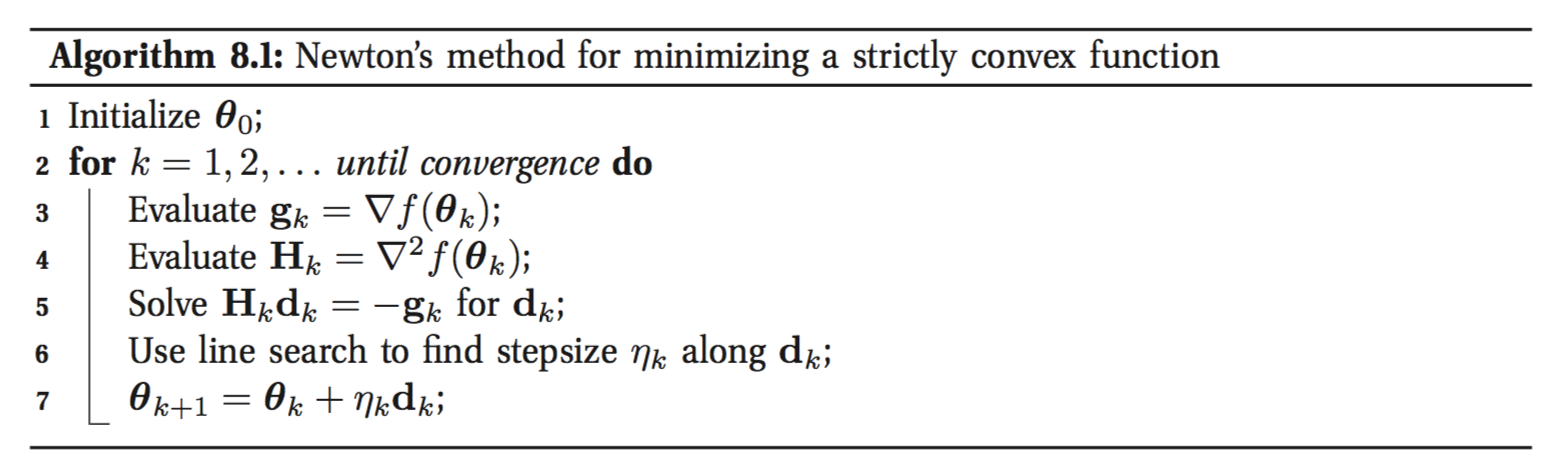
\includegraphics[width=\linewidth]{./images/newtons_method.png}
\end{figure}

皆さんご存知のテイラー展開によると,関数 $f(\vx)$ の $\hat\vx$ 周りでの 2 次近似は
\[
  f(\vx) \simeq f(\hat\vx) + \hat\vg\trans (\vx - \hat\vx) + \frac{1}{2} (\vx - \hat\vx)\trans \hat\vH (\vx - \hat\vx)
\]
\begin{align*}
  \hat\vg & = \nabla f \big|_{\vx = \hat\vx} \\
  \hat\vH & = \nabla^2 f \big|_{\vx = \hat\vx}
\end{align*}
である.さらに簡便な表記に直すと
\[
  f(\vx) \simeq \vx\trans \vA \vx + \vb\trans \vx + \mathrm{const.}
\]
\begin{align*}
  \vA & = \frac{1}{2} \hat\vH \\
  \vb & = \hat\vg - \hat\vH \hat\vx 
\end{align*}
となる.
最小となる $\vx_{min}$ の満たすべき停留条件 $f^\prime(\vx) = 0$ より
\begin{align*}
  2 \vA \vx_{min} + \vb & = \vzero \\
  \vx_{min} & = - \frac{1}{2} \vA\inv \vb \\
  & = - \hat\vH\inv (\hat\vg - \hat\vH \hat\vx) \\
  & = \hat\vx - \hat\vH\inv \hat\vg 
\end{align*}
\begin{embedbox}
今まで頻繁に目にしてきた最急降下法が
\[
  \vx_{\mathrm{next}} = \hat\vx - \hat\vg
\]
で与えられる1次微分だけを使った反復最適化だったのに対し,ニュートン--ラフソン法では2次微分まで用いることでより効率的に反復最適化することができる.
\end{embedbox}

\subsubsection*{線形回帰モデル}

線形回帰モデルに対して,ニュートン--ラフソン法を用いてみる.

\begin{equation}
  \vw^{\text{(new)}} = \vw^{\text{(old)}} - \vH\inv \nabla E(\vw)
\end{equation}
線形回帰モデル $y_n = \vw\trans\vphi_n$ の二乗和誤差関数
\[
  E(\vw) = \frac{1}{2} \sum_{n = 1}^N (\vw\trans\vphi_n - t_n)^2
\]
における勾配とヘッセ行列はそれぞれ
\begin{align}
  \nabla E(\vw) &= \sum_{n=1}^N (\vw\trans\vphi_n - t_n) \vphi_n \notag \\
  & = \pmatrixin{\vphi_1,\dots,\vphi_N} \pmatrixin{\vphi_1\trans \vw - t_1 \\ \vdots \\ \vphi_N\trans \vw - t_N} \notag \\
  & = \mPhi\trans \parens{\mPhi\vw - \vt} \notag \\
  & = \mPhi\trans \mPhi \vw - \mPhi\trans \vt \\
  \vH & = \sum \vphi_n \vphi_n\trans \notag \\
  & = \pmatrixin{\vphi_1,\dots,\vphi_N} \pmatrixin{\vphi_1\trans \\ \vdots \\ \vphi_N\trans} \notag \\
  & = \mPhi\trans \mPhi
\end{align}
である.

\paragraph{やってみよう} $\nabla E(\vw)$ と $\vH$ は,$E(\vw)$ を行列の形に直してから微分すると簡単に求まる.
\vspace{9em}

\paragraph{やってみよう} このとき,ニュートン--ラフソン法による $\vw$ の更新は次の式で与えられる.

